\section{Contribution \& validation}
\label{sec:intro:contrib}

In this thesis, we argue that modern modelling frameworks should consider uncertainty and time as first-class concepts.
In this dissertation, I present two contributions that support this vision.
First, we define a language with uncertainty at a first-class citizen: \langName.
We detail this contribution in~\Cref{chapt:aintea}.
Second, we define a \gls{metamodel}, and we formalise it, of the knowledge of \glspl{adptSyst}.
We present this contribution in~\Cref{chapt:tkm}.

\paragraph{\langName{}: Managing Data Uncertainty at the Language Level}
\begin{figure}
	\centering
	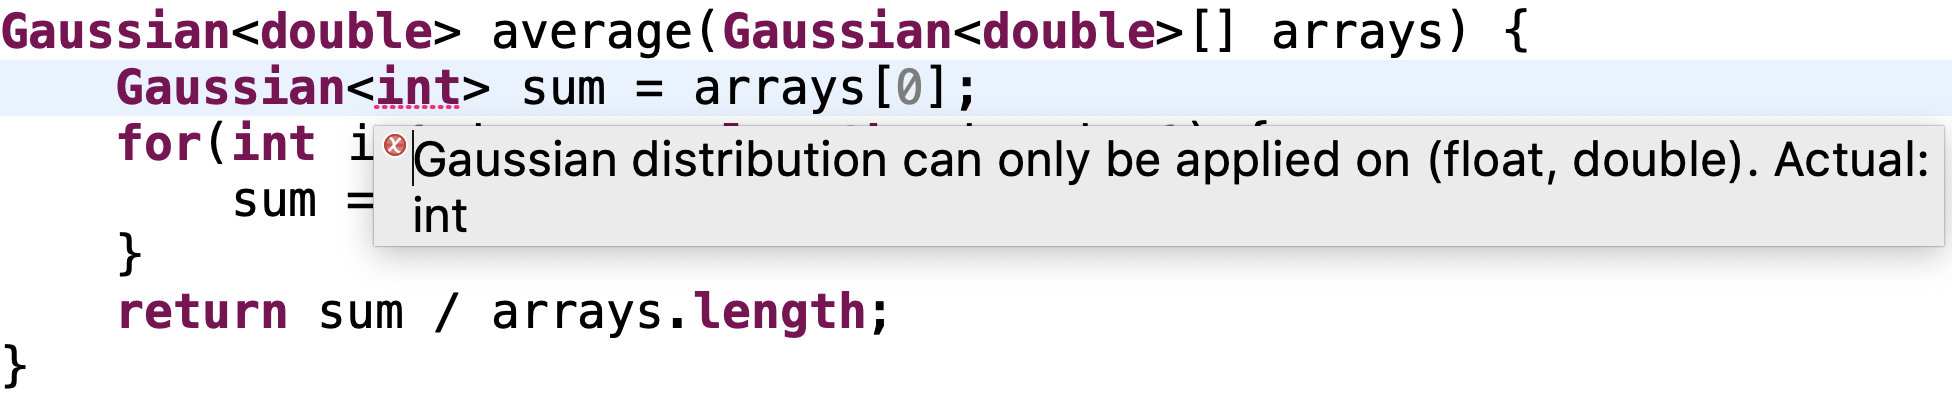
\includegraphics[width=\linewidth]{img/chapt-intro/approach/aintea-overview}
	\caption{Overview of the language proposed, \langName{}}
	\label{fig:intro:contrib:aintea}
\end{figure}

This contribution addresses the challenge of the manipulation of uncertain data (cf. Sub-Challenge \#1). 
We propose \langName{}, a language able to represent uncertain data as built-in language types along with their supported operations.
An overview of the language is depicted in~\Cref{fig:intro:contrib:aintea}.
 It contains a sampling of distributions (Gaussian, Bernoulli, binomial, Dirac delta function, and Rayleigh) that covers the different data types (booleans, numbers, and references).
 We implement a prototype of the language, publicly available on GitHub\footnote{\url{https://github.com/lmouline/aintea/}}.
 We use a real-world case study based on \gls{sg}, built with our partner Creos S.A..
It shows first that our approach does not impact the conciseness of the language.
Second, it highlights the feasibility and the advantages of uncertainty-aware type checking systems on the language level.

This contribution is under submission at the JOT Journal\footnote{\url{http://www.jot.fm/}}:
\begin{itemize}
	\item \citetitle{insubmission:2019:comlan:datauncertainty}, \citeauthor{insubmission:2019:comlan:datauncertainty}
\end{itemize}

\paragraph{A temporal knowledge \gls{metamodel}}
\begin{figure}
	\centering
	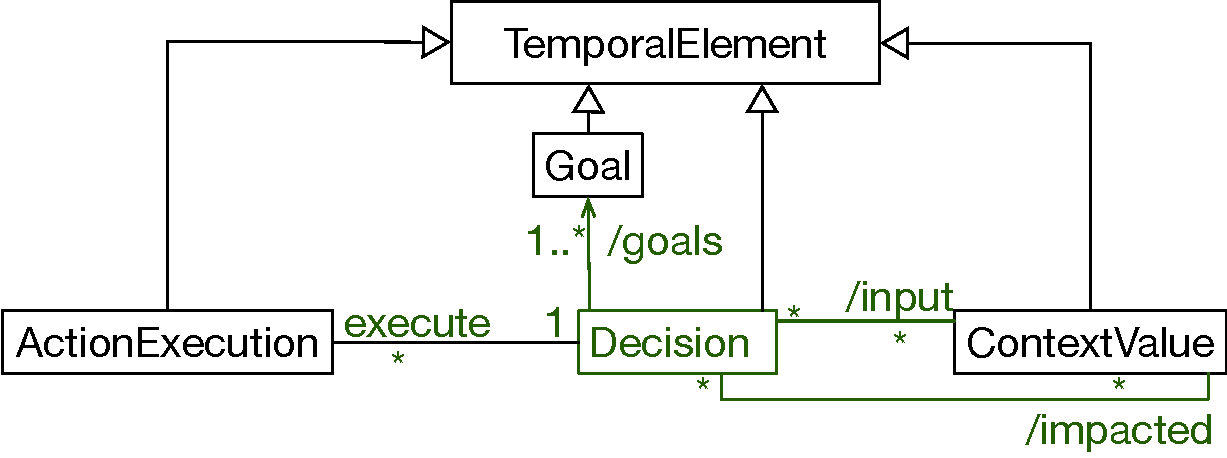
\includegraphics[width=0.6\linewidth]{img/chapt-intro/approach/tkm-overview}
	\caption{Overview of the temporal knowledge model}
	\label{fig:intro:contrib:tkm}
\end{figure}

This contribution addresses the challenge of reasoning over unfinished actions, and understanding of \gls{adptSyst} \gls{behaviour} (cf. Sub-Challenge \#2 and \#3).
First, we formalise the common core concepts implied in adaptation processes, also referred to as \gls{knowledge}.
The formalisation is based on temporal graphs and a set of relations that trace decision impacts to circumstances.
Second, we propose a framework to structure and store the state and behaviour of a running \gls{adptSyst}, together with a high-level \gls{api} to efficiently perform diagnosis routines.
Our framework relies on a temporal model-based solution that efficiently abstracts decisions, their corresponding circumstances, and their effects.
We give an overview of the \gls{metamodel} in~\Cref{fig:intro:contrib:tkm}.
We demonstrate the applicability of our approach by applying it to a \gls{sg} based example.
We also show that our approach can be used to diagnose the behaviour of at most the last five days of a district in the Luxembourg \gls{sg} in $\sim$2.4 seconds.


Part of this contribution has been published at the IEEE International Conference on Autonomic Computing\footnote{\url{http://icac2018.informatik.uni-wuerzburg.de/}} (ICAC) and at the ACM/SIGAPP Symposium On Applied Computing\footnote{\url{http://www.sigapp.org/sac/sac2018/}} (SAC):
\begin{itemize}
	\item \citetitle{DBLP:conf/sac/MoulineB0FBMB18}, \citeauthor{DBLP:conf/sac/MoulineB0FBMB18}
	\item \citetitle{DBLP:conf/icac/MoulineBFBB18}, \citeauthor{DBLP:conf/icac/MoulineBFBB18}
\end{itemize}